\chapter{Background Theory - Fluid Dynamics}
\label{chap:Theory-CFD}
\section{Problem Definition}
The objective of the thesis is to develop a GNN-based surrogate model to understand the jet deflection caused by Coanda effect in a High-speed Orienting Momentum with Enhanced Reversibility (HOMER) nozzle (cite) which is used for aerospace and industrial applications. The HOMER nozzle is designed to produce a controllable and selective deviation of a synthetic jet generated by mixing two primitive jets, without requiring any mechanical part but solely by taking advantage of the Coanda effect. The general construction of the nozzle is depicted in \ref{fig:nozzle}. As we can see from the figure, the nozzle has two inlets fed by two impinging jets followed by a convergence zone or septum where mixing of the flows occurs. The mixing of flows generates a synthetic outflow jet, which can be controlled by modifying the momentums of the primitive jets. Next to the convergence zone is the outflow mouth with curved walls connected to two convex Coanda surfaces on the top and bottom.

\begin{figure}[ht]
  \centering
  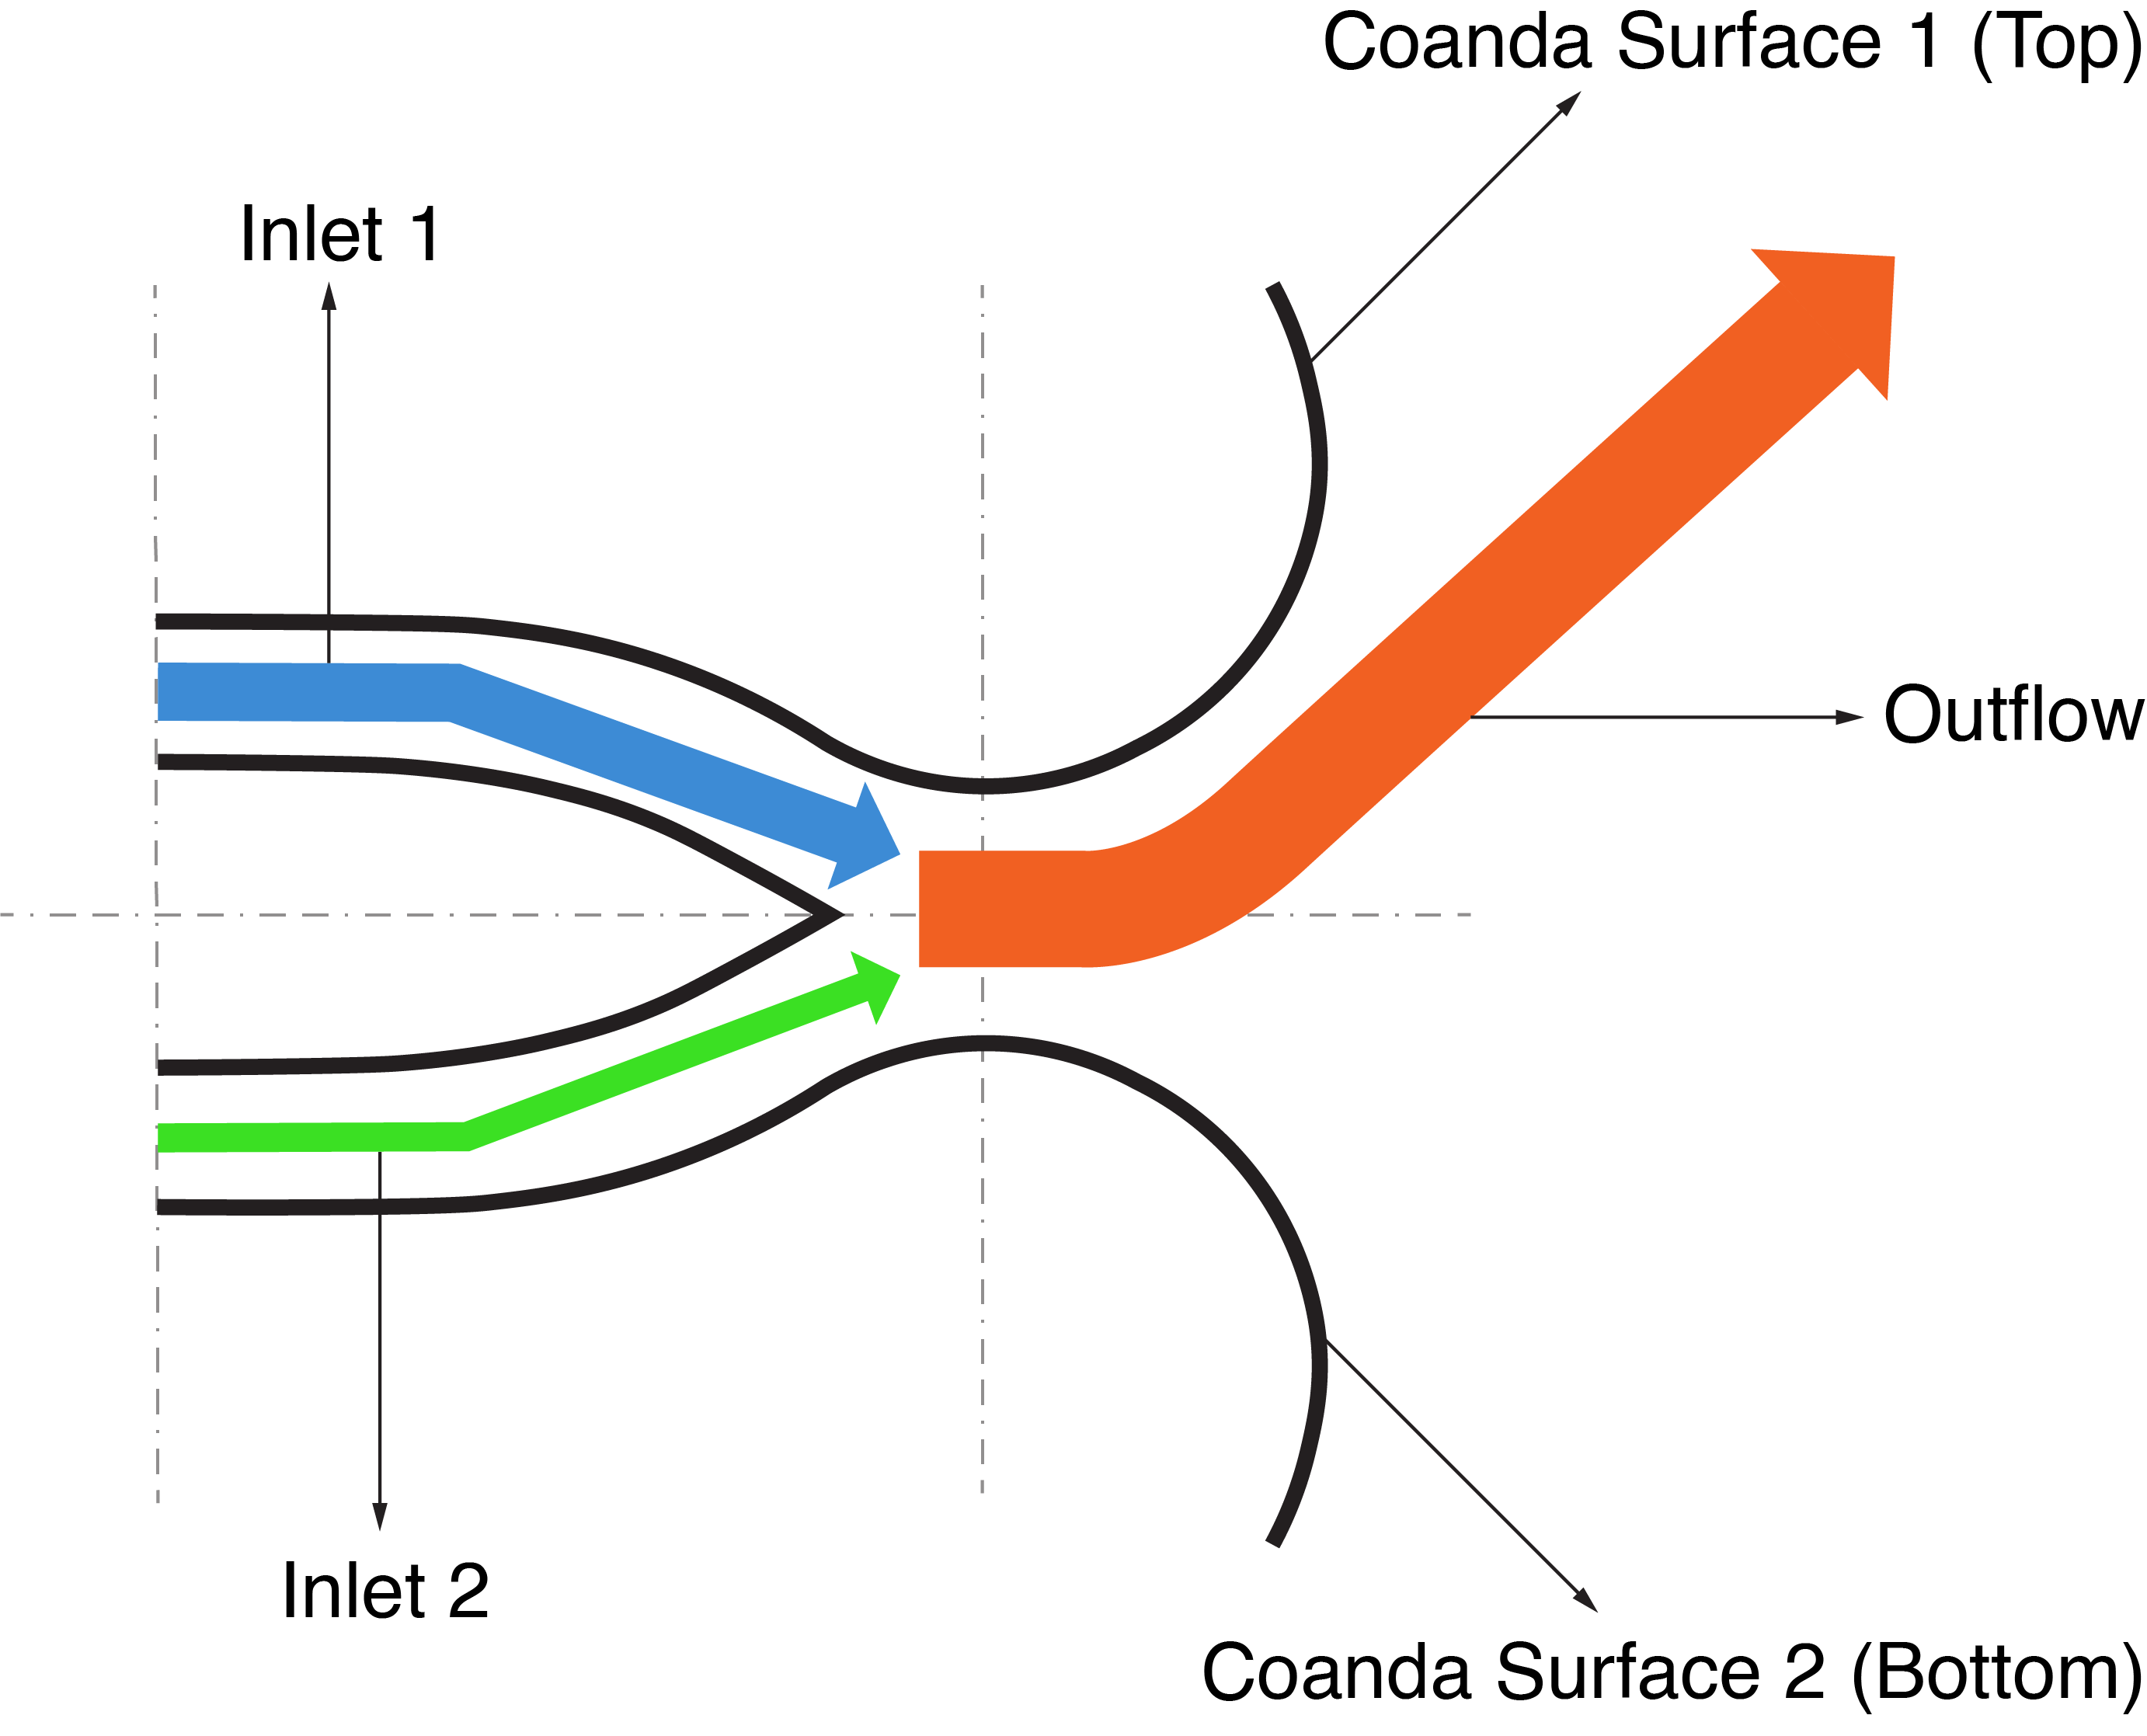
\includegraphics[width=10cm]{images/Theory-CFD/nozzle.png}
  \caption{Nozzle Architecture}
  \label{fig:nozzle}
\end{figure}

The system requires a minimum operating condition of the primitive jets to ensure effective mixing. The impinging jets must have velocities high enough to generate a synthetic jet of Reynolds number greater than 50000 at the outlet mouth. To guaranteee optimum operation, The Reynolds number at the outlet must exceed 10000. In the case of lower Reynolds numbers the system behavior is unpredictable. 
\subsection{Coanda Jet Deflection in the HOMER nozzle}
The Coanda effect is the tendency of a stream of fluid emerging from an orifice to follow an adjacent flat or curved surface and to entrain fluid from the surroundings so that a region of lower pressure develops. In simple terms, it is the tendency of a fluid to adhere to and stay attached to the walls of a convex surface, which is demonstrated in \ref{fig:Coanda}. Different fluid dynamic effects concur to create the so called “Coanda effect”. In particular it has been completely formulated in 1936 [2] as the combination of three effects: the boundary layer effect, the tendency of a fluid jet approaching a curved surface to remain attached to the surface; the adhesion effect, the ability of a fluid jet to adhere to a nearby surface; the attraction effect, the tendency of jet flows over convex curved surfaces to attract surrounding fluid and increase more rapidly than that of plane wall jets. Newman [3] has investigated a two-dimensional, incompressible, turbulent jet flowing around a circular cylinder. The experimental set used by Newman is shown in Figure 1. It has demonstrated that Coanda adhesion to a curved surface is a direct consequence of the balance of the forces applied on the fluid. During adhesive motion on a curved wall, they are centrifugal force and radial pressure. As the jet exit from the slot, the contact pressure with the curved wall is lower than ambient pressure because of the presence of viscous drag phenomena which are generated by the interaction of the fluid and the curved wall. This differential pressure is the main case of the fluid movement in contact with curved wall surface. The surface pressure along the curved wall rises and gradually equates the ambient pressure. In this condition there is a detachment between the curved wall and the fluid jet. In real viscous flows the engagement of the fluid jet with a curved wall cause an increased jet thickness proceeding along the contact with a decrease of mean velocity, because of an adverse pressure gradient. Inviscid flows may attach themselves according to the balance of centrifugal forces, but viscous effects are the cause for jet separation from the curved wall.
\begin{figure}[ht]
    \centering
    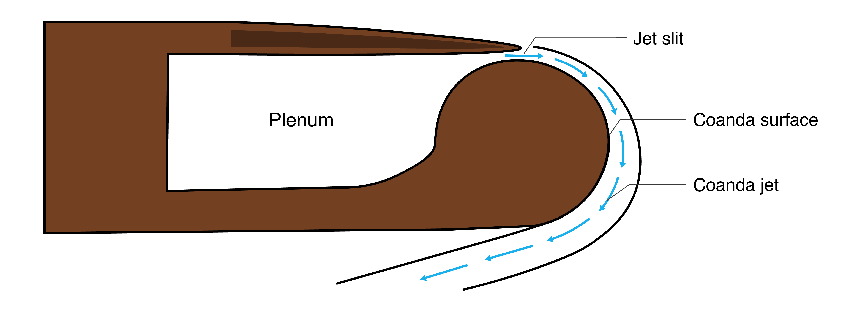
\includegraphics[width=10cm]{images/Theory-CFD/Coanda-effect.png}
    \caption{Coanda Effect}
    \label{fig:Coanda}
  \end{figure}
\section{Flow Simulation}
\ref{fig:Domain} shows the computational domain for our fluid flow problem. We consider the same homogenous fluid for both the primitive jets, that is streams with the same chemical and physical properties ($\rho$ = constant).
\begin{figure}[ht]
  \centering
  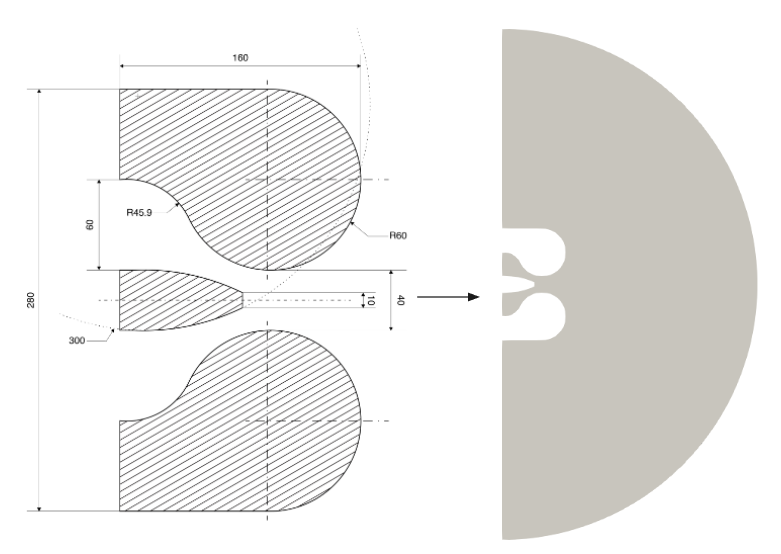
\includegraphics[width=10cm]{images/Theory-CFD/Flow Domain.png}
  \caption{Computational Flow Domain}
  \label{fig:Domain}
\end{figure}